%%%%%%%%%%%%%%%%%%%%%%%%%%%%%%%%%%%%%%%%%
% fphw Assignment
% LaTeX Template
% Version 1.0 (27/04/2019)
%
% This template originates from:
% https://www.LaTeXTemplates.com
%
% Authors:
% Class by Felipe Portales-Oliva (f.portales.oliva@gmail.com) with template 
% content and modifications by Vel (vel@LaTeXTemplates.com)
%
% Template (this file) License:
% CC BY-NC-SA 3.0 (http://creativecommons.org/licenses/by-nc-sa/3.0/)
%
%%%%%%%%%%%%%%%%%%%%%%%%%%%%%%%%%%%%%%%%%

%----------------------------------------------------------------------------------------
%	PACKAGES AND OTHER DOCUMENT CONFIGURATIONS
%----------------------------------------------------------------------------------------

\documentclass[
	12pt, % Default font size, values between 10pt-12pt are allowed
	%letterpaper, % Uncomment for US letter paper size
	%spanish, % Uncomment for Spanish
]{../Template/fphw}

% Template-specific packages
\usepackage[utf8]{inputenc} % Required for inputting international characters
\usepackage[T1]{fontenc} % Output font encoding for international characters
\usepackage{mathpazo} % Use the Palatino font

\usepackage{graphicx} % Required for including images

\usepackage{booktabs} % Required for better horizontal rules in tables

\usepackage{listings} % Required for insertion of code

\usepackage{enumerate} % To modify the enumerate environment

% Additional packages needed
\usepackage{amsmath}
\usepackage{enumitem}
\usepackage{mwe}
\usepackage{comment}
\usepackage{algorithm}
\usepackage{algpseudocode}
\usepackage{tikz}

% --- Macros ---
\newcommand{\x}{\mathbf{x}}
\renewcommand{\b}{\mathbf{b}}
\newcommand{\y}{\mathbf{y}}
\newcommand{\h}{\mathbf{h}}
\renewcommand{\a}{\mathbf{a}}
\newcommand{\W}{\mathbf{W}}
\newcommand{\g}{\mathbf{g}}



%----------------------------------------------------------------------------------------
%	ASSIGNMENT INFORMATION
%----------------------------------------------------------------------------------------

\title{Homework \#2} % Assignment title

\author{Mao Nishino} % Student name

\date{February 29th, 2024} % Due date

\institute{Florida State University \\ Department of Computer Science} % Institute or school name

\class{Deep and Reinforcement Learning Fundamentals (CAP5619-0001.sp24)} % Course or class name

\professor{Dr. Xiuwen Liu} % Professor or teacher in charge of the assignment

%----------------------------------------------------------------------------------------

\begin{document}

\maketitle % Output the assignment title, created automatically using the information in the custom commands above

%----------------------------------------------------------------------------------------
%	ASSIGNMENT CONTENT
%----------------------------------------------------------------------------------------

\section*{Problem 1}

\begin{problem}
 For a fully connected multiple-layer perceptron neural network described in Algorithms 6.3 and
6.4, where the L2 regularization of all the weights and biases is used as the regularization term ($\Omega(\theta)$).
\begin{enumerate}[label=(\arabic*)]
    \item Give the number of addition operations, number of multiplication operations, and the number of activation
function calculations for Algorithm 6.3. You need to express your answers in terms of columns and rows of the
weight matrices and the length of bias vectors. Furthermore, we assume the square of x is done by x * x.
    \item As in (1), give the numbers of addition operations, multiplication operations, and activation function calculations for Algorithm 6.4.
\end{enumerate}
Note that the addition and multiplication operations needed for activation function calculations are included implicitly
in the number of activation function calculations and should not be included as additional addition and multiplication
operations.
\end{problem}

%------------------------------------------------

\subsection*{Answer}
We collect important facts to solve this problem.
\begin{itemize}
    \item Let $x,y\in \mathbb{R}^n$. For the inner product calculation $x^T y$, The number of multiplication operations needed is $n$, and the number of addition operations needed is $n-1$ (The first element does not need summation).
    \item Let $A\in \mathbb{R}^{m\times n}$(the set of $m\times n$ real matrices) and $x\in \mathbb{R}^n$. For the matrix-vector product calculation $Ax$, The number of multiplication operations needed is $mn$, and the number of addition operations needed is $m(n-1)$ since we repeat inner product calculations for the number of rows $m$.
    \item Let $x\in \mathbb{R}^{m}$ and $y\in \mathbb{R}^{n}$. For the vector-vector outer product $xy^{T}$, The number of multiplications needed is $mn$ (since the elements of $xy^T$ are of the form $x_i y_j$).
\end{itemize}

\begin{enumerate}[label=(\arabic*)]
    \item Let us first review the setting for Algorithm 6.3. This algorithm takes a single input vector $\x$ and conducts the forward propagation computation through a fully connected MLP, finally calculating the loss. For completeness, we restate the algorithm in Algorithm \ref{alg:6.2}.

    \begin{algorithm}
    \caption{Algorithm 6.3 from the textbook}\label{alg:6.2}
        \begin{algorithmic}
            \Require Network depth, $l$
            \Require $\W^{(i)}, i\in \{1,\cdots, l\}$, the weight matrices of the model
            \Require $\b^{(i)}, i\in \{1,\cdots,l\}$, the bias parameters of the model
            \Require $\x$, the input to process
            \Require $\y$, the target output
            \State $\h^{(0)} =\x$
            \For{$k=1,\cdots ,l$}
                \State $\a^{(k)} = \b^{(k)} +\W^{(k)}\h^{(k-1)}$
                \State $\h^{(k)} = f(\a^{(k)})$
            \EndFor
            \State $\hat{\y} = \h^{(l)}$
            \State $J=L(\hat{\y},\y)+\lambda \Omega(\theta)$
        \end{algorithmic}
    \end{algorithm}
We need to define each layer's input and output sizes to answer this question. We define the input size of the $k$th layer ($k=1,\cdots ,l$) as $n^{(k-1)}$, and the output size as $n^{(k)}$. This means that the shape of $\W^{(k)}$ is $n^{(k)}\times n^{(k-1)}$ and the one for $\h^{(k)}$ is $n^{(k)}$. Moreover, the number of all parameters is $\sum_{k=1}^{l}n^{(k)}(n^{(k-1)}+1)$. By using this notation and the facts stated at the beginning, we have the following:
\begin{itemize}
    \item For each $k$, to calculate $\W^{(k)}\h^{(k-1)}$, we need $n^{(k)}n^{(k-1)}$ multiplications and $n^{(k)}(n^{(k-1)}-1)$ additions.
    \item Following that, adding $\b^{(k)}\in \mathbb{R}^{n^{(k)}}$ and $\W^{(k)}\h^{(k-1)}\in \mathbb{R}^{n^{(k)}}$ requires $n^{(k)}$ additions.
    \item Finally, the calculation of $f(\a^{(k)})$ where $\a^{(k)}\in \mathbb{R}^{n^{(k)}}$ requires $n^{(k)}$ activation calculations.
\end{itemize}
Therefore, at each $k$, we need $n^{(k)}n^{(k-1)}$ multiplications, $n^{(k)}(n^{(k-1)}-1) + n^{(k)} = n^{(k)}n^{(k-1)}$ additions, and $n^{(k)}$ activations. Now, at the end of the calculation, We need to calculate $\Omega(\theta)=\theta^T \theta$, where $\theta$ is a $\sum_{k=1}^{l}n^{(k)}(n^{(k-1)}+1)$-dimensional vector containing all parameters. This means that the number of multiplications needed here is $\sum_{k=1}^{l}n^{(k)}(n^{(k-1)}+1)$ and the number of additions needed is $\sum_{k=1}^{l}n^{(k)}(n^{(k-1)}+1)-1$. Then, we need to multiply $\Omega$ by $\lambda$ and add the loss and the regularization parameter, which increases the number of multiplications and additions by $1$, respectively. Overall, we have:
\begin{itemize}
    \item The number of multiplication operations needed is $\sum_{k=1}^{l}n^{(k)}n^{(k-1)}+\sum_{k=1}^{l}n^{(k)}(n^{(k-1)}+1)+1 = 2\sum_{k=1}^{l}n^{(k)}n^{(k-1)}+\sum_{k=1}^{l}n^{(k)}+1 $. 
    \item The number of addition operations needed is $\sum_{k=1}^{l}n^{(k)}n^{(k-1)}+\sum_{k=1}^{l}n^{(k)}(n^{(k-1)}+1)-1+1 = 2\sum_{k=1}^{l}n^{(k)}n^{(k-1)} + \sum_{k=1}^{l}n^{(k)}$
    \item The number of activation function calculations is $\sum_{k=1}^{l}n^{(k)}$.
\end{itemize}

\item We will use the same notation $n^{(k)}$ for the shape of parameters. We again restate Algorithm 6.4 for convenience.

\begin{algorithm}
    \caption{Algorithm 6.4 from the textbook}\label{alg:6.4}
    \begin{algorithmic}
        \State After the forward computation, compute the gradient on the output layer:
        \State $\g \leftarrow \nabla_{\hat{\y}} J = \nabla_{\y}L(\hat{\y},\y)$
        \For{$k=l,l-1,\cdots, 1$}
        \State Convert the gradient on the layer's output into a gradient on the pre-nonlinearly activation (element-wise multiplication if $f$ is element-wise):
        \State $\g \leftarrow \nabla_{\a^{(k)}}J = \g\odot f'(\a^{(k)})$
        \State Compute gradients on weights and biases (including the regularization term, where needed):
        \State $\nabla_{b^{(k)}} J = \g + \lambda \nabla_{\b^{(k)}} \Omega (\theta)$ 
        \State $\nabla_{\W^{(k)}} = \g {\h^{(k-1)}}^T + \lambda \nabla_{\W^{(k)}}\Omega (\theta)$
        \State Propagate the gradients w.r.t. the next lower-level hidden layers' activations:
        \State $\g\leftarrow \nabla_{\h^{(k-1)}}J = {\W^{(k)}}^{T} \g$
        \EndFor
    \end{algorithmic}
\end{algorithm}
 We will see line by line. At each $k$, we note that $\g$ is $n^{(k)}$-dimensional vector. Therefore,
\begin{itemize}
    \item As $\a^{(k)}\in \mathbb{R}^{n^{(k)}}$, the evaluation of $f'(\a^{(k)})$ requires $n^{(k)}$ activations. Then, the elementwise multiplication with $\g \in \mathbb{R}^{n^{(k)}}$ requires $n^{(k)}$ multiplications. 
    \item Since $\nabla_{\b^{(k)}}\Omega (\theta) = 2\b^{(k)}\in \mathbb{R}^{n^{(k)}}$, the evaluation of $\lambda \nabla_{\b^{(k)}} \Omega (\theta)$ costs us $2n^{(k)}$ multiplications($\times 2$ and $\times \lambda$), and it is followed by $n^{(k)}$ additions to evaluate $\nabla_{b^{(k)}} J = \g + \lambda \nabla_{\b^{(k)}} \Omega (\theta)$.
    \item $\g {\h^{(k-1)}}^T$ is an outer product between $n^{(k)}$ and $n^{(k-1)}$ dimensional vectors, so we need $n^{(k)}n^{(k-1)}$ multiplications to evaluate this. On the other hand, since $\nabla_{\W^{(k)}}\Omega (\theta) = 2 \W^{(k)}$, we need $2n^{(k)}n^{(k-1)}$ multiplications to evaluate $\lambda \nabla_{\W^{(k)}}\Omega (\theta)$, and it is followed by $n^{(k)}n^{(k-1)}$ additions to evaluate $\g {\h^{(k-1)}}^T + \lambda \nabla_{\W^{(k)}}\Omega (\theta)$.
    \item Finally, since ${\W^{(k)}}^T\in \mathbb{R}^{n^{(k-1)}\times n^{(k)}}$, evaluating ${\W^{(k)}}^{T} \g$ requires $n^{(k)}n^{(k-1)}$ multiplications and $n^{(k-1)}(n^{(k)}-1)$ additions to evaluate it.
\end{itemize}
To summarize, we need $n^{(k)} + 2n^{(k)}+n^{(k)}n^{(k-1)}+2n^{(k)}n^{(k-1)}+n^{(k)}n^{(k-1)}= 4n^{(k)}n^{(k-1)}+3n^{(k)}$ multiplications, $n^{(k)}+n^{(k)}n^{(k-1)}+n^{(k-1)}(n^{(k)}-1) = 2n^{(k)}n^{(k-1)}+n^{(k)}-n^{(k-1)}$ additions, and $n^{(k)}$ activations in one iteration. Therefore,
\begin{itemize}
\item We need $\sum_{k=1}^{l}\left(4n^{(k)}n^{(k-1)}+3n^{(k)}\right)$ multiplication operations,
\item $\sum_{k=1}^{l}\left(2n^{(k)}n^{(k-1)}+n^{(k)}-n^{(k-1)}\right)$ addition operations, and
\item $\sum_{k=1}^{l}n^{(k)}$ activation function calculations.
\end{itemize}

\end{enumerate}

%----------------------------------------------------------------------------------------

\section*{Problem 2}

\begin{problem}
     Answer the following questions regarding L2 and L1 regularization, and early stopping.
     \begin{enumerate}[label = (\arabic*)]
        \item Explain intuitively why L2 regularization is known as weight decay. Then explain how it is related to early
        stopping.
        \item Explain intuitively why L1 regularization leads to more parameter sparsity (i.e., more parameter values are small
        and close to zero) than L2 regularization.
        \item Compared to Algorithm 7.1, what is the main advantage of Algorithms 7.2 and 7.3? Briefly explain.
    \end{enumerate}
\end{problem}

%------------------------------------------------

\subsection*{Answer}

\begin{enumerate}[label = (\arabic*)] % Sub-questions styled as italic letters
	\item Consider a generic loss function with the $L^2$ penalty term: $J(\theta)= L(\theta)+\frac{\alpha}{2} \theta^{T} \theta$ where $\theta$ is the vector of parameters to train. The gradient of $J$ with respect to $\theta$ is 
    \begin{equation}
        \nabla_{\theta} J = \nabla_{\theta} L + \alpha \theta 
    \end{equation}
    Therefore, the update formula of $\theta$ using the gradient descent with the learning rate $\eta$ is 
    \begin{align}
        \theta^{(n+1)} &= \theta^{(n)} - \eta\left(\nabla_{\theta} L + \alpha \theta^{(n)} \right) \\
        &= (1-\eta \alpha )\theta^{(n)} - \eta \nabla_{\theta}L
    \end{align}
    where we can observe the weight decay $(1-\eta \alpha )\theta^{(n)}$. More intuitively, see Figure \ref{fig:l2reg} and its caption for a graphical explanation. 
    \begin{figure}[!htbp]
    \centering
\tikzset{every picture/.style={line width=0.75pt}} %set default line width to 0.75pt        

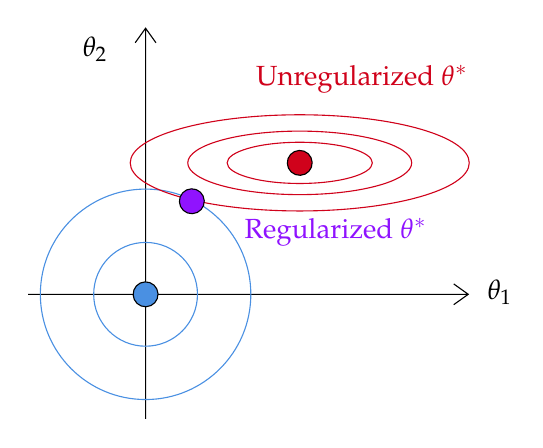
\begin{tikzpicture}[x=0.75pt,y=0.75pt,yscale=-1,xscale=1]
%uncomment if require: \path (0,194); %set diagram left start at 0, and has height of 194

%Shape: Axis 2D [id:dp21131980094580838] 
\draw  (227,130) -- (439,130)(283.54,1.8) -- (283.54,190) (432,125) -- (439,130) -- (432,135) (278.54,8.8) -- (283.54,1.8) -- (288.54,8.8)  ;
%Shape: Circle [id:dp08810116721807959] 
\draw  [color={rgb, 255:red, 74; green, 144; blue, 226 }  ,draw opacity=1 ] (258.54,130) .. controls (258.54,116.19) and (269.73,105) .. (283.54,105) .. controls (297.35,105) and (308.54,116.19) .. (308.54,130) .. controls (308.54,143.81) and (297.35,155) .. (283.54,155) .. controls (269.73,155) and (258.54,143.81) .. (258.54,130) -- cycle ;
%Shape: Circle [id:dp8544668398661346] 
\draw  [color={rgb, 255:red, 74; green, 144; blue, 226 }  ,draw opacity=1 ] (232.84,130) .. controls (232.84,102) and (255.54,79.3) .. (283.54,79.3) .. controls (311.54,79.3) and (334.24,102) .. (334.24,130) .. controls (334.24,158) and (311.54,180.7) .. (283.54,180.7) .. controls (255.54,180.7) and (232.84,158) .. (232.84,130) -- cycle ;
%Shape: Circle [id:dp49929007834143424] 
\draw  [fill={rgb, 255:red, 208; green, 2; blue, 27 }  ,fill opacity=1 ] (351.82,66.94) .. controls (351.67,63.63) and (354.23,60.82) .. (357.54,60.67) .. controls (360.85,60.53) and (363.66,63.09) .. (363.8,66.4) .. controls (363.95,69.71) and (361.39,72.52) .. (358.08,72.66) .. controls (354.77,72.81) and (351.96,70.25) .. (351.82,66.94) -- cycle ;
%Shape: Circle [id:dp8861753216380706] 
\draw  [fill={rgb, 255:red, 74; green, 144; blue, 226 }  ,fill opacity=1 ] (277.55,130.27) .. controls (277.4,126.96) and (279.96,124.15) .. (283.27,124.01) .. controls (286.58,123.86) and (289.39,126.42) .. (289.53,129.73) .. controls (289.68,133.04) and (287.12,135.85) .. (283.81,135.99) .. controls (280.5,136.14) and (277.69,133.58) .. (277.55,130.27) -- cycle ;
%Shape: Ellipse [id:dp14045537271083375] 
\draw  [color={rgb, 255:red, 208; green, 2; blue, 27 }  ,draw opacity=1 ] (322.82,66.67) .. controls (322.82,61.19) and (338.48,56.74) .. (357.81,56.74) .. controls (377.14,56.74) and (392.8,61.19) .. (392.8,66.67) .. controls (392.8,72.15) and (377.14,76.6) .. (357.81,76.6) .. controls (338.48,76.6) and (322.82,72.15) .. (322.82,66.67) -- cycle ;
%Shape: Ellipse [id:dp8820312380580158] 
\draw  [color={rgb, 255:red, 208; green, 2; blue, 27 }  ,draw opacity=1 ] (303.86,66.67) .. controls (303.86,58.22) and (328.02,51.37) .. (357.81,51.37) .. controls (387.6,51.37) and (411.76,58.22) .. (411.76,66.67) .. controls (411.76,75.12) and (387.6,81.97) .. (357.81,81.97) .. controls (328.02,81.97) and (303.86,75.12) .. (303.86,66.67) -- cycle ;
%Shape: Ellipse [id:dp8381773996506672] 
\draw  [color={rgb, 255:red, 208; green, 2; blue, 27 }  ,draw opacity=1 ] (276.14,66.67) .. controls (276.14,53.87) and (312.7,43.5) .. (357.81,43.5) .. controls (402.92,43.5) and (439.48,53.87) .. (439.48,66.67) .. controls (439.48,79.46) and (402.92,89.84) .. (357.81,89.84) .. controls (312.7,89.84) and (276.14,79.46) .. (276.14,66.67) -- cycle ;
%Shape: Circle [id:dp9542321948034993] 
\draw  [fill={rgb, 255:red, 144; green, 19; blue, 254 }  ,fill opacity=1 ] (299.83,85.43) .. controls (299.68,82.12) and (302.25,79.32) .. (305.56,79.17) .. controls (308.87,79.02) and (311.67,81.58) .. (311.82,84.89) .. controls (311.96,88.21) and (309.4,91.01) .. (306.09,91.16) .. controls (302.78,91.3) and (299.98,88.74) .. (299.83,85.43) -- cycle ;

% Text Node
\draw (335.5,18.4) node [anchor=north west][inner sep=0.75pt]  [color={rgb, 255:red, 208; green, 2; blue, 27 }  ,opacity=1 ]  {$\text{Unregularized } \theta ^{*}$};
% Text Node
\draw (330,91.9) node [anchor=north west][inner sep=0.75pt]  [color={rgb, 255:red, 208; green, 2; blue, 27 }  ,opacity=1 ]  {$\textcolor[rgb]{0.56,0.07,1}{\text{Regularized } \theta ^{*}}$};
% Text Node
\draw (447,121.9) node [anchor=north west][inner sep=0.75pt]    {$\theta _{1}$};
% Text Node
\draw (252,4.9) node [anchor=north west][inner sep=0.75pt]    {$\theta _{2}$};


\end{tikzpicture}
    \caption{The figure on how $L^2$ regularization decays the parameters. We assume that our parameter is two dimensional, i.e. $\theta=(\theta_1,\theta_2)$, and that the unregularized loss $L(\theta)$ is quadratic in $\theta$. The blue concentric circles around the origin show the level curves for the $L^2$ penalty, i.e., the graph for $\theta^T \theta = k$ for some equidistant $k$s (say $k=1,2,\cdots$) and the red ellipses centered at the unregularized optimal parameter $\theta^*$ show the level curves for $L(\theta)$. The new solution is at an intersection of some of these level curves, as shown in the figure. The level curves for $L$ show that $L$ is less steep in the direction of $\theta_1$, meaning that this direction is less important, and the figure shows that $\theta^*$ is more decayed in this unimportant direction. That is, the $L^2$ penalty decays the parameters that are not important. }
    \label{fig:l2reg}
\end{figure}
    We will now focus on early stopping. We will show that the early stopping is equivalent to $L^2$ regularization for a simple linear model with a quadratic $L$ and the classical gradient descent as an update rule. Consider a linear regression model, i.e., one-layer perception with a linear activation function, and suppose the loss $L(\theta)$ is quadratic. Then, the second-order Taylor expansion is exact:
    \begin{equation}
        L(\theta) = L(\theta^*) + \frac{1}{2}(\theta-\theta^*)^T H(\theta-\theta^*)
    \end{equation}
    where $\theta^*$ is the optimal parameter and $H$ is the Hessian matrix of $L$ evaluated at $\theta^*$. We note that we have no first-order term since $\theta^*$ is optimal, $\nabla_{\theta}L(\theta^*)=0$. By taking the gradient, we have
    \begin{equation}
        \nabla_{\theta} L(\theta) = H(\theta-\theta^*)
    \end{equation}
    Therefore, the update rule using the gradient descent is 
    \begin{equation}
        \label{eqn:updaterule_HW2q2}
        \theta^{(n+1)} = \theta^{(n)} - \eta H(\theta^{(n)}-\theta^*)
    \end{equation}
    Suppose we stop the training at $n=\tau$. Rewriting the equation (\ref{eqn:updaterule_HW2q2}) shows that
    \begin{align}
        \theta^{(n+1)}-\theta^* &= (I-\eta H)(\theta^{(n)}-\theta^*)
    \end{align}
    We will now use the eigenvalue decomposition $H=Q\Lambda Q^T$ where $Q$ is the orthogonal matrix of eigenvectors, and $\Lambda$ is the diagonal matrix of eigenvectors. We have
    \begin{align}
        \theta^{(n+1)}-\theta^* &= Q(I-\eta \Lambda )Q^T(\theta^{(n)}-\theta^*) \\
        Q^T (\theta^{(n+1)}-\theta^*) &= (1-\eta \Lambda)Q^T(\theta^{(n)}-\theta^*)
    \end{align}
    Therefore
    \begin{equation}
        Q^T(\theta^{(\tau)}-\theta^*) = (I-\eta \Lambda)^{\tau}Q^T(-\theta^*)
    \end{equation}
    or
    \begin{equation}
        Q^T\theta^{(\tau)} = [I-(I-\eta\Lambda)^{\tau}]Q^T\theta^*
    \end{equation}
    assuming the initial parameter is zero. We use that (without proof) the solution to the $L^2$ regularized problem $\tilde{\theta}$ satisfies
    \begin{align}
        Q^T \tilde{\theta} &= (\Lambda +\alpha I)^{-1}\Lambda Q^T \theta^* \\ &=[I-(\Lambda +\alpha I)^{-1}\alpha]Q^T \theta^*
    \end{align}
    where $\alpha$ is the regularization constant. We used the algebraic formula $\frac{\lambda}{\lambda+\alpha} = 1-\frac{\alpha}{\lambda+\alpha}$. Note that both $\Lambda$ and $\alpha I$ are diagonal matrices, so this formula applies directly. Now, if we  choose $\tau, \eta$ and $\alpha$ so that $(I-\eta \Lambda)^{\tau} = (\Lambda + \alpha I)^{-1}\alpha$, we see that $\theta^{(\tau)}=\tilde{\theta}$ and $L^2$ regularization is equivalent to early stopping. At least for lower dimensional cases (such as 1D), we can easily choose $\alpha,\eta$, and $\tau$ since we have three degrees of freedom while we have only one equation.

    \item See Figure \ref{fig:l1sparse} and its caption for a graphical solution. 
    
    \begin{figure}
        \centering
        

\tikzset{every picture/.style={line width=0.75pt}} %set default line width to 0.75pt        

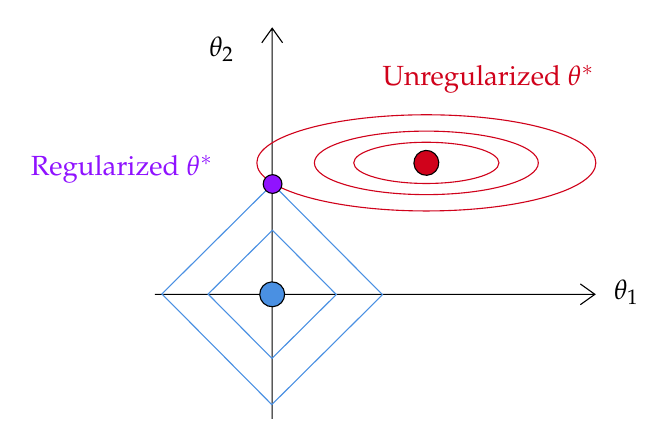
\begin{tikzpicture}[x=0.75pt,y=0.75pt,yscale=-1,xscale=1]
%uncomment if require: \path (0,194); %set diagram left start at 0, and has height of 194

%Shape: Axis 2D [id:dp24512449599942188] 
\draw  (227,130) -- (439,130)(283.54,1.8) -- (283.54,190) (432,125) -- (439,130) -- (432,135) (278.54,8.8) -- (283.54,1.8) -- (288.54,8.8)  ;
%Shape: Circle [id:dp31283958216444874] 
\draw  [fill={rgb, 255:red, 208; green, 2; blue, 27 }  ,fill opacity=1 ] (351.82,66.94) .. controls (351.67,63.63) and (354.23,60.82) .. (357.54,60.67) .. controls (360.85,60.53) and (363.66,63.09) .. (363.8,66.4) .. controls (363.95,69.71) and (361.39,72.52) .. (358.08,72.66) .. controls (354.77,72.81) and (351.96,70.25) .. (351.82,66.94) -- cycle ;
%Shape: Circle [id:dp9878588785830922] 
\draw  [fill={rgb, 255:red, 74; green, 144; blue, 226 }  ,fill opacity=1 ] (277.55,130.27) .. controls (277.4,126.96) and (279.96,124.15) .. (283.27,124.01) .. controls (286.58,123.86) and (289.39,126.42) .. (289.53,129.73) .. controls (289.68,133.04) and (287.12,135.85) .. (283.81,135.99) .. controls (280.5,136.14) and (277.69,133.58) .. (277.55,130.27) -- cycle ;
%Shape: Ellipse [id:dp23546583238427532] 
\draw  [color={rgb, 255:red, 208; green, 2; blue, 27 }  ,draw opacity=1 ] (322.82,66.67) .. controls (322.82,61.19) and (338.48,56.74) .. (357.81,56.74) .. controls (377.14,56.74) and (392.8,61.19) .. (392.8,66.67) .. controls (392.8,72.15) and (377.14,76.6) .. (357.81,76.6) .. controls (338.48,76.6) and (322.82,72.15) .. (322.82,66.67) -- cycle ;
%Shape: Ellipse [id:dp7653976694315836] 
\draw  [color={rgb, 255:red, 208; green, 2; blue, 27 }  ,draw opacity=1 ] (303.86,66.67) .. controls (303.86,58.22) and (328.02,51.37) .. (357.81,51.37) .. controls (387.6,51.37) and (411.76,58.22) .. (411.76,66.67) .. controls (411.76,75.12) and (387.6,81.97) .. (357.81,81.97) .. controls (328.02,81.97) and (303.86,75.12) .. (303.86,66.67) -- cycle ;
%Shape: Ellipse [id:dp18063197356967042] 
\draw  [color={rgb, 255:red, 208; green, 2; blue, 27 }  ,draw opacity=1 ] (276.14,66.67) .. controls (276.14,53.87) and (312.7,43.5) .. (357.81,43.5) .. controls (402.92,43.5) and (439.48,53.87) .. (439.48,66.67) .. controls (439.48,79.46) and (402.92,89.84) .. (357.81,89.84) .. controls (312.7,89.84) and (276.14,79.46) .. (276.14,66.67) -- cycle ;
%Shape: Square [id:dp4737956643266181] 
\draw  [color={rgb, 255:red, 74; green, 144; blue, 226 }  ,draw opacity=1 ] (283.65,99.12) -- (314.42,130.11) -- (283.43,160.88) -- (252.66,129.89) -- cycle ;
%Shape: Square [id:dp22714730690690543] 
\draw  [color={rgb, 255:red, 74; green, 144; blue, 226 }  ,draw opacity=1 ] (283.73,76.86) -- (336.68,130.19) -- (283.35,183.14) -- (230.4,129.81) -- cycle ;
%Shape: Circle [id:dp2925456236616477] 
\draw  [color={rgb, 255:red, 0; green, 0; blue, 0 }  ,draw opacity=1 ][fill={rgb, 255:red, 144; green, 19; blue, 254 }  ,fill opacity=1 ] (279.21,76.89) .. controls (279.2,74.4) and (281.2,72.37) .. (283.7,72.35) .. controls (286.19,72.34) and (288.22,74.34) .. (288.24,76.83) .. controls (288.25,79.33) and (286.25,81.36) .. (283.76,81.38) .. controls (281.26,81.39) and (279.23,79.38) .. (279.21,76.89) -- cycle ;

% Text Node
\draw (335.5,18.4) node [anchor=north west][inner sep=0.75pt]  [color={rgb, 255:red, 208; green, 2; blue, 27 }  ,opacity=1 ]  {$\text{Unregularized } \theta ^{*}$};
% Text Node
\draw (166,61.9) node [anchor=north west][inner sep=0.75pt]  [color={rgb, 255:red, 208; green, 2; blue, 27 }  ,opacity=1 ]  {$\textcolor[rgb]{0.56,0.07,1}{\text{Regularized }}\textcolor[rgb]{0.56,0.07,1}{\theta }\textcolor[rgb]{0.56,0.07,1}{^{*}}$};
% Text Node
\draw (447,121.9) node [anchor=north west][inner sep=0.75pt]    {$\theta _{1}$};
% Text Node
\draw (252,4.9) node [anchor=north west][inner sep=0.75pt]    {$\theta _{2}$};


\end{tikzpicture}
        \caption{The figure on how $L^1$ regularization can produce sparsity. The setting is the same as Figure \ref{fig:l2reg}, but the level curves for the $L^2$ penalty term are now replaced by the one for the $L^1$ penalty term. Due to its characteristic shape, which emphasizes its vertices, it is more likely to intersect at them, which produces sparse solutions. Indeed, in this example, the optimal solution has $\theta_1=0$.}
        \label{fig:l1sparse}
    \end{figure}
    \item The major difference between Algorithm 7.1 and the subsequent algorithms is that 7.1 uses the validation set only to calculate the error and is not used for training. On the other hand, 7.2 and 7.3 fully utilize this extra data for training once the early stopping criterion is found.
\end{enumerate}

%----------------------------------------------------------------------------------------

\section*{Problem 3}

\begin{problem}
Answer the following questions regarding gradient-based optimization algorithms for deep
learning.
\begin{enumerate}[label=(\arabic*)]
\item Explain the pros and cons of small and large minibatch sizes in Algorithm 8.1. Here we assume GPU memory
is sufficiently large.
\item Explain how the momentum term in Algorithm 8.2 helps overcome plateau regions and speed up learning in
regions where the non-zero gradients are roughly constant.
\item Explain when and how the Adam algorithm in Algorithm 8.7 gives better estimation of the momentum term
than the basic momentum algorithm in Algorithm 8.2.
\item Explain how the learning rates are adaptive in Algorithms 8.4 and 8.5.
\end{enumerate}


\end{problem}

%------------------------------------------------

\subsection*{Answer} 
\begin{enumerate}[label = (\arabic*)]
\item By using larger mini-batches, the pros are that we can approximate the gradient more accurately and utilize parallel computation to speed up the calculation. For the cons, the larger size often shows poor generalization ability. The pro of the smaller mini-batches is that they offer better generalization due to the noise they add to the training process. The cons are that the gradient estimate will have a high variance, meaning we need to choose a lower learning rate, leading to a longer runtime.
\item The updating equations of the SGD with momentum are as follows:
\begin{align}
    v^{(n+1)} &= \alpha v^{(n)} - \eta g \label{eqn:momentum} \\
    \theta^{(n+1)} &= \theta^{(n)}+v^{(n)}
\end{align}
where $v$ is the momentum, $g$ is the gradient and $\theta$ is the parameter of a neural network. We observe that the momentum $v$ accumulates the past gradients by Equation (\ref{eqn:momentum}). Therefore, even if we end up in the plateau region where the gradient $g$ is close to $0$, the accumulated gradient from $v$ will help us move in such a region. Now, suppose that the gradient $g$ is roughly constant. Then, in the equilibrium ($n\to \infty$), Equation (\ref{eqn:momentum}) becomes
\begin{equation}
    v^{(\infty)} = \frac{-\eta g}{1-\alpha}
\end{equation}
This equation shows that the usual step size $-\eta g$ is multiplied by $\frac{1}{1-\alpha}$ when we use the momentum. For example, if $\alpha=0.99$, the momentum is $100$ times faster than the usual gradient descent when the gradient is roughly constant.
\item What corresponds to momentum in the Adam algorithm is the estimation of the first moment. In both the usual momentum and the Adam, the momentum or the first moment is initialized by zero. According to \cite{adam}, this causes the estimate to be biased towards zero. To correct the bias, the Adam algorithm divides the updated estimation by $1-\rho_1^t$, where $\rho_1$ is a hyperparameter and $t$ is the time step. \cite{adam} notes that the uncorrected estimation is especially biased when the decay rate is low (i.e., $\rho_1$ is close to 1, so the gradient decay is small) Therefore, the bias correction provided by Adam should provide a better estimate than the classical momentum method in this situation.

\item In both the AdaGrad algorithm (Algorithm 8.4) and the RMSProp algorithm (Algorithm 8.5), the central trick is to accumulate the squared gradient. In AdaGrad, we sum up all the squared gradients in the current and past steps, and in RMSProp, we do the same, but we gradually decay the past gradients. Then, we use this accumulated square gradient $r$ to divide the learning rate used in the gradient descent step. According to the textbook, in the AdaGrad algorithm, the learning rate is changed to be $\frac{\epsilon}{\delta+\sqrt{r} }$ and in RMSProp, it is $\frac{\epsilon}{\sqrt{\delta+r}}$ where $\epsilon$ is the original learning rate and $\delta$ is a small parameter to avoid zero division. Since $r$ is a vector, the division above should be seen as an elementwise operation, meaning we have different learning rates for each parameter. The parameters with larger gradients would have a lower learning rate, stabilizing the learning, and the ones with smaller gradients would have a larger learning rate, promoting faster learning.

\end{enumerate}
%----------------------------------------------------------------------------------------

\section*{Problem 4}

\begin{problem}
A central problem in machine learning (including deep learning) is how to make
an algorithm that perform well not just on the training data, but also on new inputs. Two techniques that are shown to
be effective empirically are dropout and batch normalization, even though the underlying mechanisms are not well
entirely clear.
\begin{enumerate}[label=(\arabic*)]

\item What are the expected side effects of dropout, where additional noise is introduced by randomly removing
neurons during training?
\item Dropout is often regarded as an efficient way to implement bagging. Identify and explain the differences
between bagging and dropout.
\item What are the expected side effects of batch normalization, where normalization reduces the expressive power
of the involved layers?
\item While it is well defined how to perform normalization during the training phase on a minibatch (see equations
(8.36) and (8.37) in the Deep Learning textbook), what to do at the test time is not clearly defined. Explain
expected undesirable side effects.
\item Based on your understanding, explain how dropout and batch normalization should be used jointly.
\end{enumerate}
\end{problem}

%------------------------------------------------

\subsection*{Answer}
\begin{enumerate}[label = (\arabic*)]
    \item First, it can increase the training time due to the noise affecting the gradient. Second, according to the textbook, since Dropout is a regularization technique, it reduces the capacity of the model. We need to increase the model size to mitigate this effect, and the increased computational cost might be too expensive to justify the use of Dropout. Moreover, we will have a hyperparameter (the dropout probability) to tune, which would complicate the training. Finally, \cite{liang2021rdrop} mentions that there is an inconsistency between the model in training (some nodes are dropped out) and the model in inference (all nodes are present), which hinders the model performance.

    \item In Bagging, we create multiple models trained on different training sets, and each model is independent, meaning that no parameters are shared between each model. In Dropout, while multiple models are created by dropping out some nodes and trained on different training sets (minibatches), they are not independent and share the parameters. This allows us to simulate exponentially many different models without requiring exponentially large memory. Moreover, in Bagging, we typically train each model completely to the convergence, but this is not the case for Dropout. In fact, most models are not explicitly trained at all since we only pick up a fraction of them randomly. It would still work well because of the parameter sharing, which allows us to train models we didn't choose.

    \item Although batch normalization was introduced to mitigate the covariate shift, where the distribution of the input for each layer changes constantly, it has a few desirable and undesirable side effects. First, it has a regularization effect because of the noise introduced by the normalization operation. Since minibatches are chosen randomly, their mean and the variance naturally contain some randomness, which improves the regularization. Second, it can reduce the training time. On the other hand, due to its regularization effect, it can reduce the capacity of the model, but the textbook offers a way to avoid this by introducing new parameters scaling the normalized result. It also requires larger batch sizes for stable mean and variance estimation. Indeed, \cite{groupnorm} reports that reducing the batch size increases the model error dramatically.

    \item According to the text, we use the moving average of means and the variance to normalize at the test time to allow an evaluation for a single sample. However, this is inconsistent with the behavior at the training, and \cite{failurebn} mentions that this causes Transformer models with batch normalization to perform poorly in NLP tasks.

    \item The original paper \cite{batchnorm} states that since batch normalization acts as a regularizer, we can sometimes remove Droput for performance. In fact, \cite{doandbn} states that they often perform poorly when used together. \cite{doandbn} explains that the reason is due to \textit{variance shift}, which is caused by the change of variance of output coming from Dropout between the test and the training phase. To avoid this, the authors suggest two strategies: (1) Applying Dropout after all BN layers, and (2) Modify Dropout so that it is less prone to variance shift. For (2), they introduce the \textit{Uout} method, where instead of dropping out, we transform the input $x_i$ by $X=x_i+x_i r_i$ where $r_i$ follows the uniform distribution on $(-\beta, \beta)$ and $\beta$ is a hyperparameter. 
\end{enumerate}


%----------------------------------------------------------------------------------------
\begin{thebibliography}{9}
\bibitem{adam}
Kingma, D. P., \& Ba, J. (2017). Adam: A Method for Stochastic Optimization. arXiv:1412.6980. https://arxiv.org/abs/1412.6980

\bibitem{liang2021rdrop}
Liang, X., Wu, L., Li, J., Wang, Y., Meng, Q., Qin, T., Chen, W., Zhang, M., \& Liu, T.-Y. (2021). R-Drop: Regularized Dropout for Neural Networks. arXiv. https://arxiv.org/abs/2106.14448

\bibitem{groupnorm} Wu, Y., \& He, K. (2018). Group Normalization. arXiv:1803.08494. https://arxiv.org/abs/1803.08494

\bibitem{failurebn} Wang, J., Wu, J., \& Huang, L. (2022). Understanding the Failure of Batch Normalization for Transformers in NLP. arXiv. arXiv:2210.05153.

\bibitem{batchnorm}Ioffe, S., \& Szegedy, C. (2015). Batch Normalization: Accelerating Deep Network Training by Reducing Internal Covariate Shift. arXiv:1502.03167. https://arxiv.org/abs/1502.03167

\bibitem{doandbn}Li, X., Chen, S., Hu, X., \& Yang, J. (2018). Understanding the Disharmony between Dropout and Batch Normalization by Variance Shift. arXiv:1801.05134. https://arxiv.org/abs/1801.05134



\end{thebibliography}

\end{document}
